%\begin{figure}[t!]
%	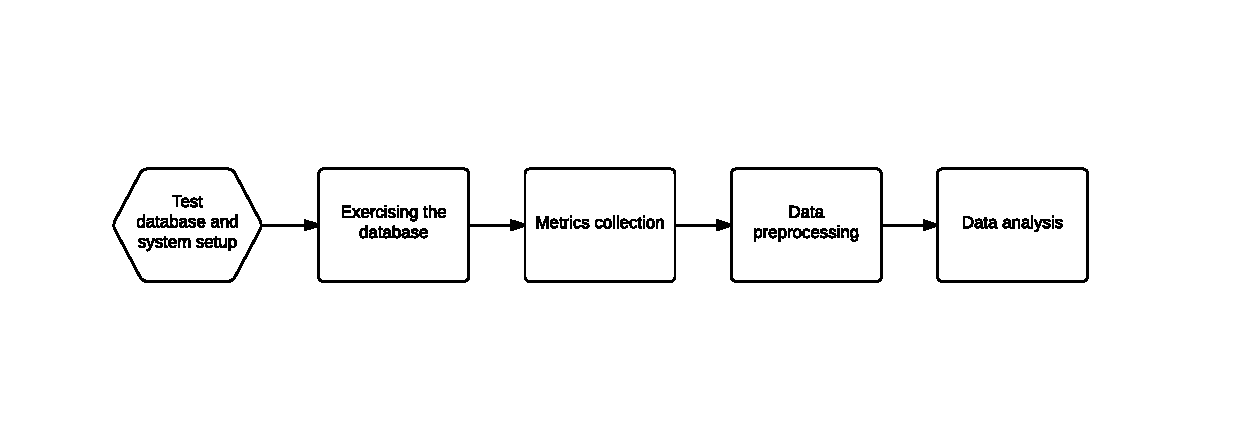
\includegraphics[width=1\textwidth]{approach.pdf}
%	\centering
%	\caption{Approach overview}
%    \label{fig:approach}
%\end{figure} 
%%\includepdf][pages={1}][width=\columnwidth{approach.pdf}

\begin{figure}[thb]
	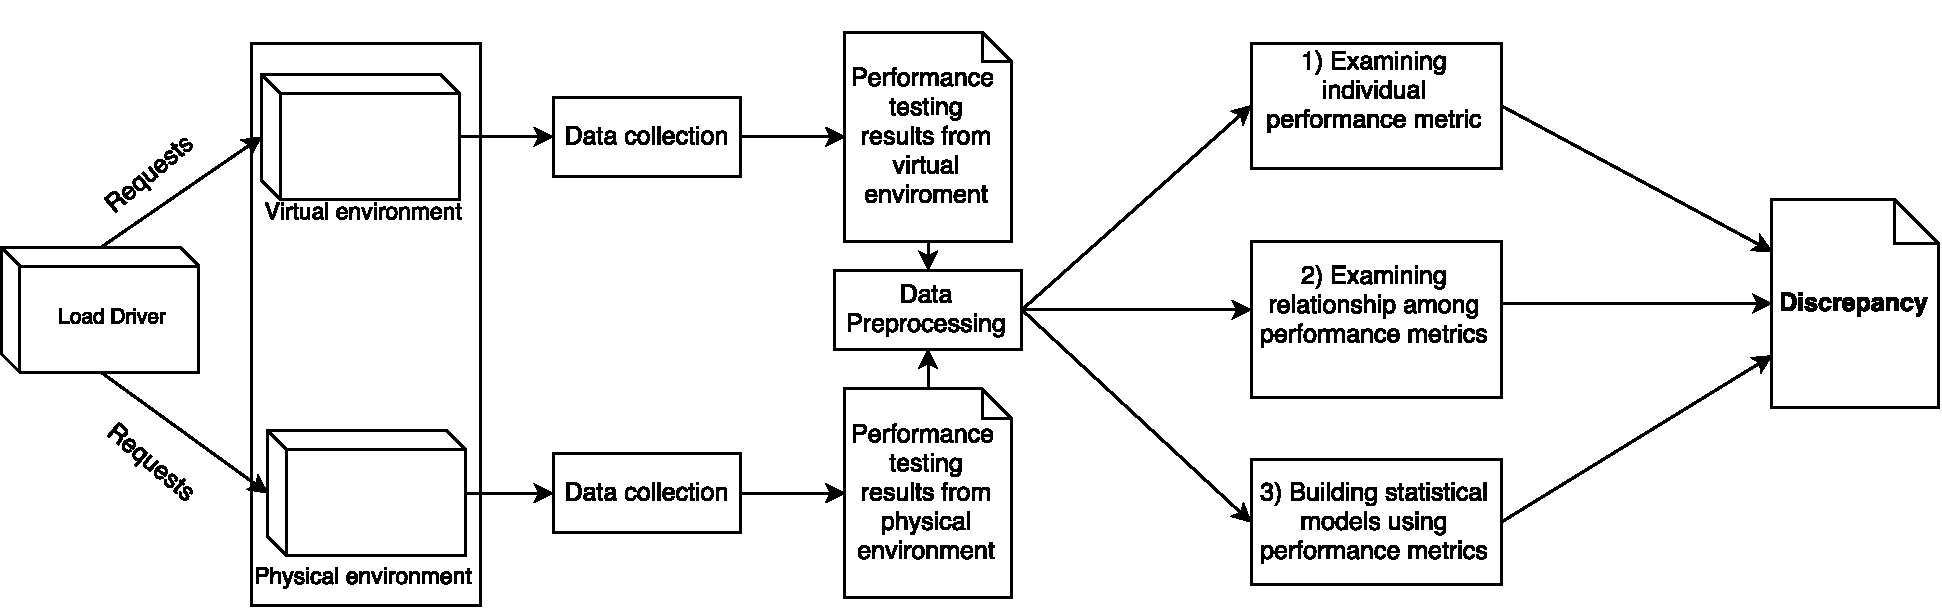
\includegraphics[width=.9\textwidth]{overview}
	\caption{An overview of our case study setup.}
	%\captionsetup{justification=centering}
	\label{fig:Approach}
\end{figure}

The goal of our case study is to evaluate the discrepancy between performance testing results from virtual and physical environments. We deploy our subject systems in two identical environments(physical and virtual). A load driver is used to exercise our subject systems. After the collection and processing of the performance metrics we analyze and draw conclusions based on: 1) individual performance metrics 2) relationship among performance metrics and 3) statistical models based on the performance metrics. An overview of our case study setup is shown in Figure~\ref{fig:Approach}.


\subsection{Subject Systems}
Dell DVD Store (DS2)~\cite{delldvd} is an online multi-tier e-commerce web application that is widely used in performance testing and prior performance engineering research~\cite{Shang:2015:ADP:2668930.2688052,Nguyen:2012:ADP:2188286.2188344, jackicsm2009}. We deploy DS2 on an Apache (Version 3.0.0) web application server with MySQL 5.6 database server~\cite{mysql}. CloudStore~\cite{cloudstore}, our second subject system is an open source application based on the TPC-W benchmark~\cite{tpcw}. CloudStore is widely used to evaluate the performance of cloud computing infrastructure when hosting web-based software systems and is leveraged in prior research~\cite{tarekmsr16}. We deploy CloudStore on \textit{Apache Tomcat}~\cite{tomcat} (version 7.0.65) with MySQL 5.6 database server~\cite{mysql}. 


\subsection{Environmental Setup}

The performance tests of the two subject systems are conducted on three machines in a lab environment. Each machine has an Intel i5 4690 Haswell Quad-Core 3.50 GHz CPU, with 8 GB of memory, connected to a local gigabyte ethernet. The first machine hosts the web server and application server (Apache and Tomcat). The second machine hosts the MySQL 5.6 database server. The load drivers were deployed on the third machine. We separate the load driver, the web/application server and the database server on different machines in order to mimic real world scenario and avoid interference among these processes. For example, isolating the web and database driver would ensure that the processor is not overused. The operating systems on the three machines are Windows 7. We disable all other processes and unrelated system services to minimize their performance impact. Since our goal is to compare performance metrics in virtual and physical environments, we setup the two different environments, which we detail next.

%was dedicated to the database server, the second machine was dedicated to the web server and the third machine was used to run the load driver.
\noindent \textbf{Virtual environment.} We install one Virtual Box (version 5.0.16) and create only one virtual machine on one physical machine to avoid the interference between virtual machines. For each virtual machine, we allocate two cores and three gigabytes of memory, which is well below capacity to make sure we are topping out and pushing our configuration for unrealistic results. 

%Our virtual setup was identical to our physical setup. The virtual environment was run on the same physical machines with all the resources provided to the host and the same set of aforementioned configuration for the virtual environment. We opted for single tenancy of the guest operating system to avoid any unwanted noise. 

\noindent \textbf{Physical environment.} To make the physical environment similar to the virtual environment, we only enable two cores and 3GB memory for each machine for the physical environment. 

%To make the systems' configuration identical prior to exercising the subject systems, we chose 2 cores and 3GB of memory dedicated to each environment to avoid crashes on the guest operating system in the virtual environment. We also made sure to kill all the processes before we start our performance testing to minimize any discrepancy present.

%\subsection{Exercising the database}
%Following the set up of our subject systems on the respective servers, the systems were exercised with an aid of drivers. These drivers generated multi-type web requests and simulated real-time user behavior depending on the input parameters provided. We ran our performance tests for numerous hours while recording all the performance metrics generated for varying load applied on our software systems.
\subsection{Performance tests}

DS2 is released with a dedicated load driver program that is designed to exercise DS2 for performance testing. We used the load driver to conduct performance testing on DS2. We used Apache JMeter~\cite{apachejmeter} to generate a workload to conduct the performance tests on CloudStore. For both subject systems, the workload of the performance tests is varied periodically in order to avoid bias from a consistent workload. The workload variation was introduced by the number of threads. A higher number of threads represent a higher number of users accessing the system. Each performance test is run after a 15 minute warming up period of the system and lasts for 9 hours. 


%and the last 30 minutes in order to 

 %The choice of load was random but consistent between both of the environments. As our study was based on exercising our systems and recording the performance metrics, and not stress testing \cite{stresstesting}, the respected limits were chosen in order to avoid the under-performance of the physical machine and system failure of the virtual machine.


%\subsection{Metrics Collection}
\subsection{Data collection and preprocessing}

\noindent \textbf{Performance metrics.} We used \textit{PerfMon}~\cite{perfmon} to record the values of performance metrics. \textit{PerfMon} is a performance monitoring tool used to observe and record performance metrics such as CPU utilization, memory usage and disk IOs. We record all the available performance metrics that can be monitored on a single process by \emph{PerfMon}.  We recorded the performance metrics of both the processes, web server and the database server, with an interval of 10 seconds. In total, we recorded 44 performance metrics. 

\noindent \textbf{System throughput.} We used the web server access logs from Apache and Tomcat to calculate the throughput of the system by measuring the number of requests per minute. The two data sets were then concatenated and mapped against requests using their respective timestamps.

In order to combine the two datasets of performance metrics and system throughput, and to minimize noise of the performance metric recording, we calculate the mean values of the performance metrics in every minute. Then, we combine the datasets of performance metrics and system throughput based on the time stamp on a per minute basis. A similar approach has been applied to address mining performance metrics challenges~\cite{foo2010mining}.
